As we mentionned earlier, images unlike texts have properties which lead traditional algorithm of encryption (mostly block-cypher algorithm like AES-128, RC6...) to some drawbacks. When the algorithm is applied to a pixel at the position $(x,y)$, the values of the four bytes (RGBa) change. These modifications need to appear randomly to the attackers in order to consider the algorithm as a good encryption algorithm. We can analyze the algorithm in several ways, we will present three of them here and we will apply these methods to the proposed algorithm. 

\begin{figure}[!h]	
\centering
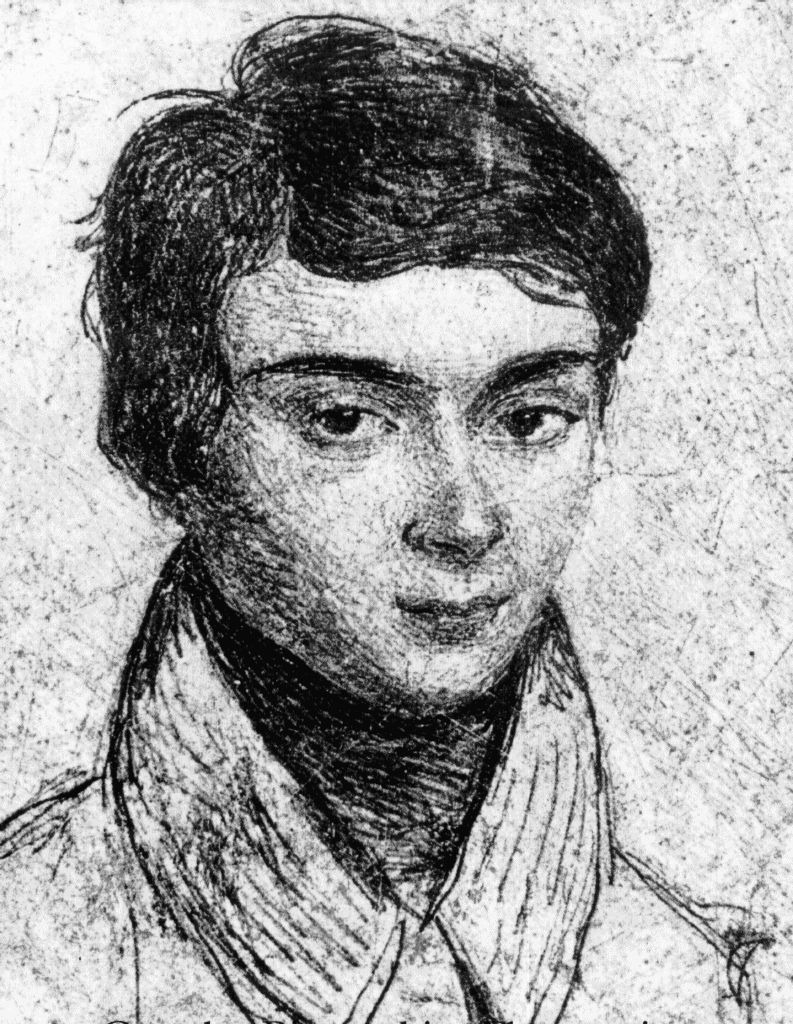
\includegraphics[scale=1.15]{tex/img/galois.jpg}
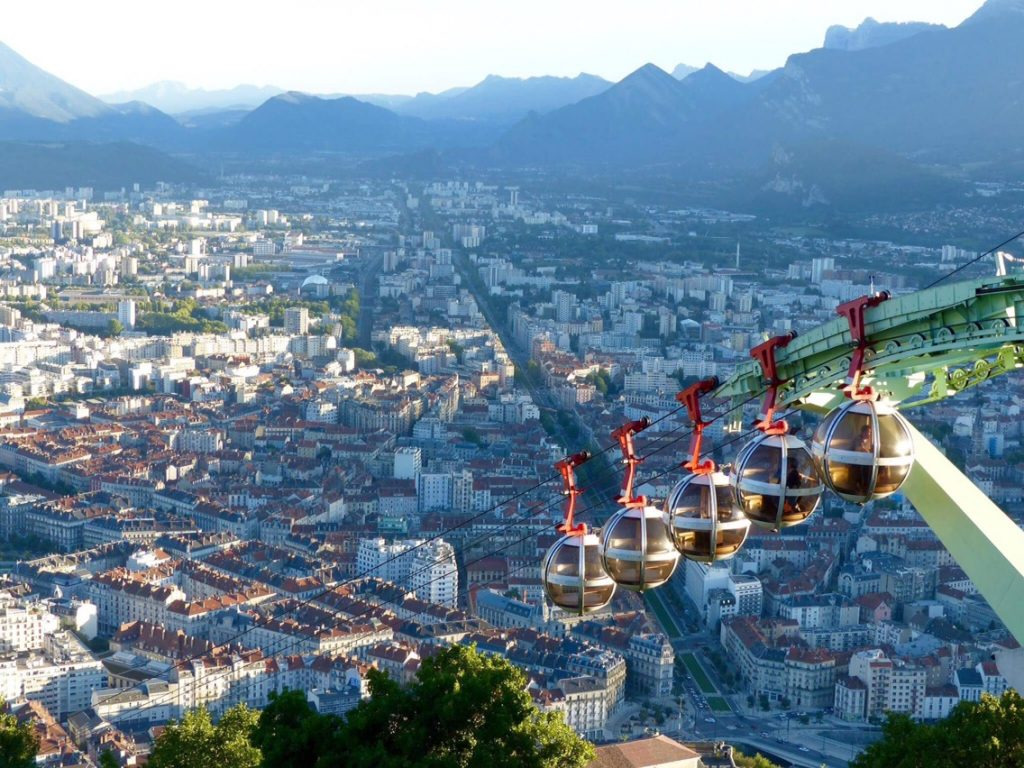
\includegraphics[scale=1.55]{tex/img/grenoble_city.jpg}
\caption{\textit{galois.bmp} and \textit{grenoble\_city.bmp} used for the analysis of the proposed algorithm}
\end{figure}

In order to test the proposed algorithm of the \textit{Section 2}, we are going to encrypt two images : \textbf{galois.bmp} and \textbf{grenoble\_city.bmp}. The first one is a black and white image encoded as an RGBa image, this is interesting because this lead the Red byte, the Green and the Blue one to be equal and the alpha byte set at 255. The second one is a picture of the city of Grenoble in France encoded as an RGBa image. \\
